\chapter{Leap Motion controller}\label{LMCChapter}

\section{Controller}
Leap Motion is an USB sensor device released in July 2013 by Leap Motion Inc., designed to provide realtime tracking of hands and fingers in three-dimensional space with 0.01 milimeter accuracy. It allows a user to get information about objects located in device's field of view (about 150 degree with distance not exceeding 1 meter).
%https://www.leapmotion.com/press_releases/leap-motion-to-launch-leap-motion-controller-exclusively-at-best-buy]. 

Details of how Leap Motion performs 3D scene capturing have not been revealed by Leap Motion, Inc. However, it is known that hardware consists of three infrared LEDs which are used for scene illumination, while two cameras spaced 4 centimeters apart capture images with 50-200 fps framrate, dependant whether USB 2.0 or 3.0 is used.

\begin{figure}[htb]
\centering
 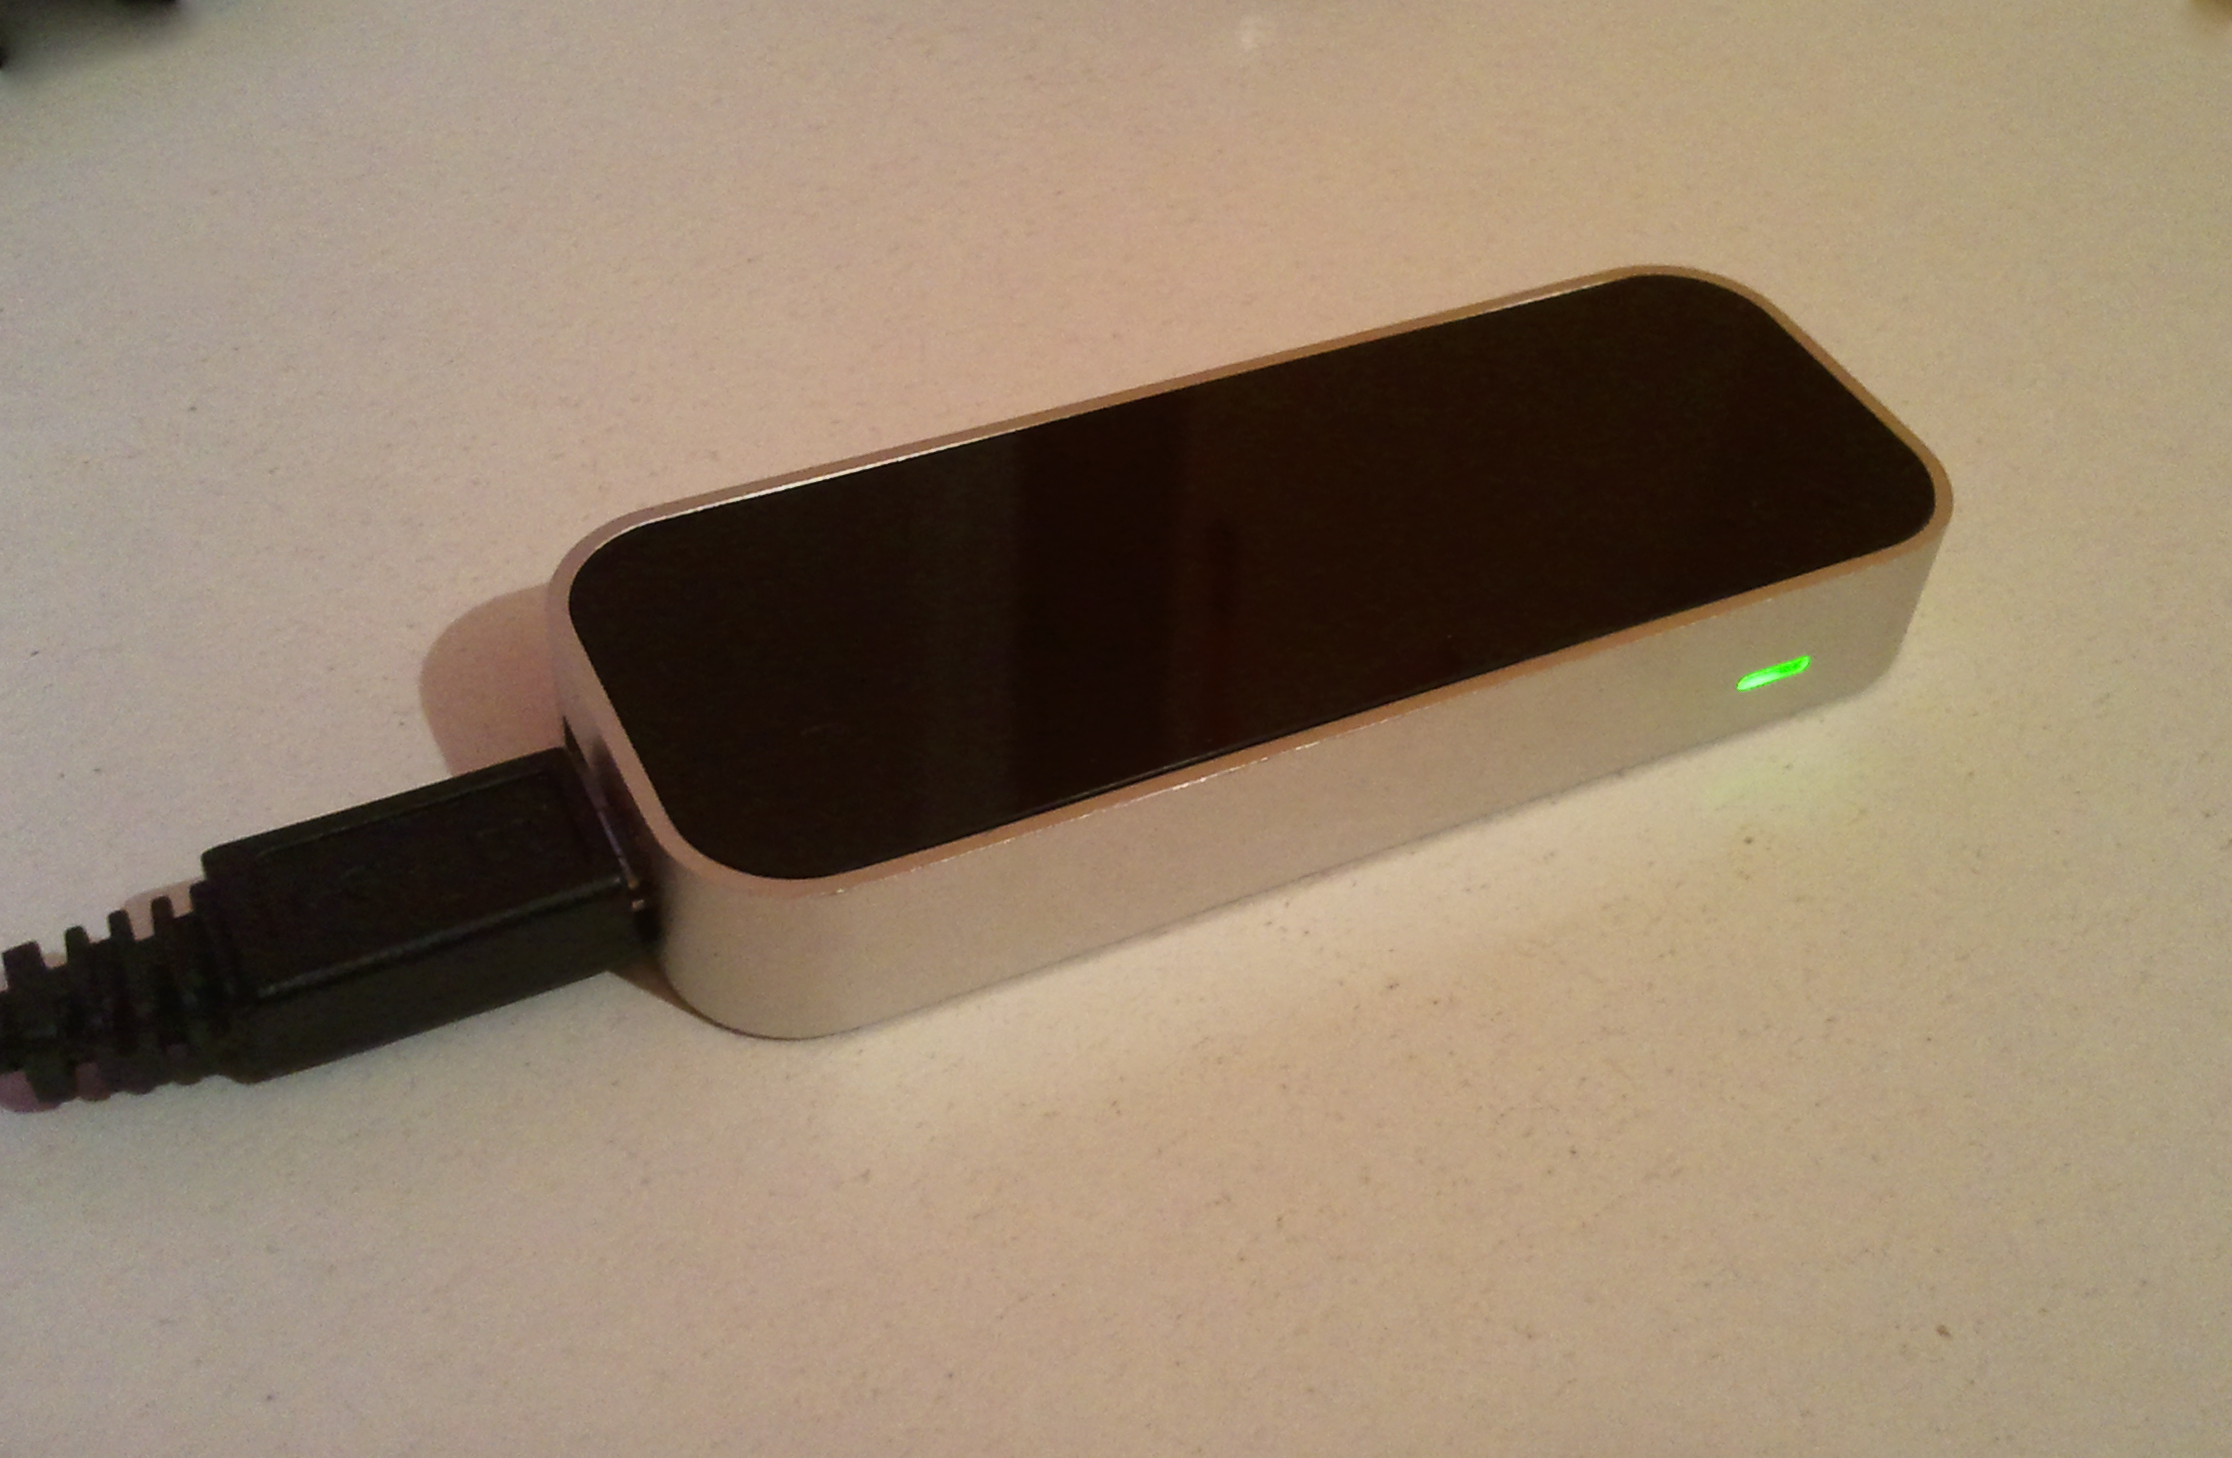
\includegraphics[width=1\columnwidth]{figures/leapmotion.jpg}
 \caption{Leap Motion controller with Micro--USB plug}
 \label{recorder}
\end{figure}

\section{Data access}

Unlike Microsoft Kinect, Leap Motion does not provide access to raw data in the form of a cloud of points. Captured data is processed by proprietary drivers supplied by vendor and accessible through API. Leap Motion was intended to be a human-computer interface, not general purpose 3D scanner, so it is optimised for recognizing human hands and pointy objects.

The main data container we get from Leap Motion API is a Frame. Average framerate while using dual core laptop and USB 2.0 interface, is 50 frames per second. One frame consists of hands, fingers, pointables (objects directly visible by controller), and additional information, like gestures recognized by simple built-in recognition mechanism, frame timestamp, rotation, translation, and scaling data. 

For purposes of this project, we have created our own data format. It contains only information necessary for us and allows to easily save captured frames to file, and read them later for processing and testing purposes.
